%!TEX program = xelatex
\documentclass{article}
\input{LaTeX-Submodule/template.tex}

% Additional packages & macros
\usepackage{subcaption}
\usepackage{stanli}

% Header and footer
\newcommand{\unitName}{Engineering Mechanics}
\newcommand{\unitTime}{Semester 1, 2022}
\newcommand{\unitCoordinator}{Dr Tuquabo Tesfamichael}
\newcommand{\documentAuthors}{\textsc{Tarang Janawalkar}}

\fancyhead[L]{\unitName}
\fancyhead[R]{\leftmark}
\fancyfoot[C]{\thepage}

% Copyright
\usepackage[
    type={CC},
    modifier={by-nc-sa},
    version={4.0},
    imagewidth={5em},
    hyphenation={raggedright}
]{doclicense}

\date{}

\begin{document}
%
\begin{titlepage}
    \vspace*{\fill}
    \begin{center}
        \LARGE{\textbf{\unitName}} \\[0.1in]
        \normalsize{\unitTime} \\[0.2in]
        \normalsize\textit{\unitCoordinator} \\[0.2in]
        \documentAuthors
    \end{center}
    \vspace*{\fill}
    \doclicenseThis
    \thispagestyle{empty}
\end{titlepage}
\newpage
%
\tableofcontents
\newpage
%
\section{Stress and Strain}
\subsection{External Forces}
Rigid bodies are subjected to external force and couple moment systems that result from the effects of gravitational,
electrical, magnetic, or contact forces. Contact forces can be surface, linear, or concentrated forces.
\subsubsection{Types of Forces}
\begin{itemize}
    \item Compressive (pushing)
    \item Tensile (pulling)
    \item Shear (sliding)
    \item Torsional (twisting)
    \item Biaxial tension
    \item Hydrostatic compression
    \item Bending (induces tension, compression and shear)
\end{itemize}
\subsection{Internal Loadings}
External forces cause internal loadings that occur in equal and opposite collinear pairs as stresses and strains.
Internal loading is associated with \textbf{stress} while \textbf{strain} is a measure of a body's deformation.

These loadings have no external effects on the body and are not included on a \textbf{Free Body Diagram} (FBD) if
the entire body is considered.

To determine the forces in each member, we can use the method of sections to represent the internal loading as external forces.
\subsection{Internal Resultant Loadings}
Although the exact distribution of the internal loading may be \textit{unknown}, we can determine the
resultant force \(\symbf{F}_R\) and resultant moment \(\left( \symbf{M}_R \right)_O\) about a point \(O\) by applying the
equations of equilibrium
\begin{align*}
    \sum \symbf{F}   & = \symbf{0}  \\
    \sum \symbf{M}_O & = \symbf{0}.
\end{align*}
\begin{figure}[H]
    \centering
    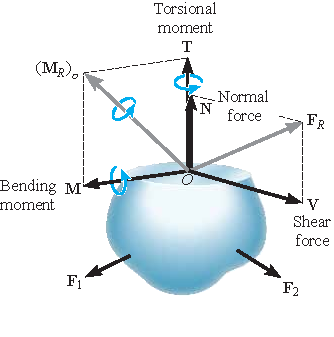
\includegraphics[height = 8cm, keepaspectratio = true]{figures/resultant_loadings.pdf}
    \caption{Resultant loadings acting on a body.}
    % \label{}
\end{figure}
\subsubsection{In 3D}
In 3D, we can represent resultant loadings using four vectors acting over the sectioned area.
\begin{description}
    \item[Normal force] \(\symbf{N}\) force acting perpendicular to the area
    \item[Shear force] \(\symbf{V}\) force acting on an axis tangent to the area
    \item[Torsional moment] \(\symbf{T}\) rotation about the perpendicular axis
    \item[Bending moment] \(\symbf{M}\) rotation about an axis tangent to the area
\end{description}
\subsubsection{In 2D}
In 2D, the body is subjected to a coplanar system of forces, where \(\symbf{T} = \symbf{0}\).
\subsubsection{In 1D}
In 1D, the body is only subjected to axial forces, where \(\symbf{V} = \symbf{T} = \symbf{M} = \symbf{0}\).
\subsection{Stress}
The force and moment acting at a specific point on a sectioned area of a body represent the resultant effects of
the distribution of internal loading that acts over the sectioned area.
\begin{definition}[Stress]
    Consider the quotient of the force \(\Delta \symbf{F}\) over an area \(\Delta A\), then as the \(\Delta A \to 0\),
    so does \(\Delta \symbf{F}\), while the quotient approaches a finite limit. This quotient is called the stress at
    that point.
    \begin{equation*}
        \symbf{\sigma} = \lim_{\Delta A \to 0} \frac{\Delta \symbf{F}}{\Delta A}
    \end{equation*}
    Here the normal and shear stresses can be expressed using \(\sigma_z\) and \(\tau_{zx}\) and \(\tau_{zy}\).
    \begin{align*}
        \sigma_z  & = \lim_{\Delta A \to 0} \frac{\Delta F_z}{\Delta A} \\
        \tau_{zx} & = \lim_{\Delta A \to 0} \frac{\Delta F_x}{\Delta A} \\
        \tau_{zy} & = \lim_{\Delta A \to 0} \frac{\Delta F_y}{\Delta A}
    \end{align*}

    Stress describes the intensity of the internal force acting on a specific region passing through a point.

    The unit for stress is Pascal where \qty{1}{Pa} or \qty{1}{N.m^{-2}} and \qty{1}{MPa} or \qty{1}{N.mm^{-2}}.
\end{definition}
To determine the average stress distribution acting over a cross-sectional area of an axially loaded bar,
we assume that the material is both \textit{homogeneous} and \textit{isotropic}.
This means the load \(P\) applied through the centroid of the cross-sectional area
will cause the bar to deform uniformly throughout the central region of its length.
\subsubsection{Average Normal Stress}
By passing a section through a bar, equilibrium requires the resultant normal force \(N\) at the section to be
equal to the external force \(P\). And because the material undergoes a uniform deformation, it is necessary
that the cross-section is subjected to a constant normal stress distribution.

As a result, each small area \(\Delta A\) on the cross section is subjected
to a force \(\Delta N = \sigma \Delta A\), where the sum of these forces over the entire cross-sectional area
is \(P\). By letting \(\Delta A \to \odif{A} \) and therefore also \( \Delta N \to \odif{N} \), then as \(\sigma\)
is a constant, we have
\begin{align*}
    \int \odif{N} & = \int_A \sigma \odif{A} \\
    N             & = \sigma A
\end{align*}
Therefore
\begin{equation*}
    \sigma_{\mathrm{avg}} = \frac{N}{A}
\end{equation*}
where in this case \(N = P\).
\begin{theorem}[Equilibrium]
    For an uniaxially loaded body, the equation of force equilibrium gives
    \begin{align*}
        \sigma \left( \Delta A \right) - \sigma' \left( \Delta A \right) & = 0       \\
        \sigma                                                           & = \sigma'
    \end{align*}
    hence the normal stress components must be equal in magnitude but opposite in direction.

    Under this condition, the material is subjected to \textbf{uniaxial stress} and this analysis
    applies to members subjected to tension or compression.
\end{theorem}
\subsubsection{Average Shear Stress}
Shear stress is the stress component that acts in the plane of the sectioned area.
Here we must consider the number of planes that are in stress due to the applied force,
so that the shear force \(V = F / n\) for \(n\) planes, is applied to hold the segment in
equilibrium.

The average shear stress distributed over each sectioned area that develops this shear force is
defined by
\begin{equation*}
    \tau_{\mathrm{avg}} = \frac{V}{A}
\end{equation*}
The loading case discussed is an example of \textbf{simple or direct shear} as the shear is caused
by the direct action of the applied load \(\symbf{F}\).
\subsection{Strain}
\begin{definition}[Deformation]
    Whenever a force is applied to a body, it will tend to change the body's shape and size.
    These changes are referred to as deformation.
\end{definition}
\begin{definition}[Strain]
    To describe the deformation of a body through changes in lengths of line segments on the surface,
    we will develop the concept of strain.
    If an axial load \(P\) is applied to a bar, it will change the bar's length \(L_0\) to \(L\).
    Then the \textbf{average normal strain} of the bar is defined
    \begin{equation*}
        \epsilon_{\mathrm{avg}} = \frac{L - L_0}{L_0}
    \end{equation*}
    where the numerator is often written as \(\delta = L - L_0\) and is known as elongation or extension.

    The \textbf{normal strain} \(\epsilon\) at a point in a body with an arbitrary shape is defined similarly.
    Consider a small line segment \(\Delta s\) which becomes \(\Delta s'\) after deformation. Then the limit of the normal strain
    is
    \begin{equation*}
        \epsilon = \lim_{\Delta s \to 0} \frac{\Delta s' - \Delta s}{\Delta s}
    \end{equation*}
    In both cases, normal strain is positive when the initial length elongates, and negative when the length contracts.

    Strain is a dimensionless quantity sometimes expressed \unit{mm/mm} or \unit{m/m}, or as a percentage.
\end{definition}
\subsection{Shear Strain}
Deformations not only cause line segments to elongate or contract, but they also cause them to change direction.
If we consider two line segments that are originally perpendicular to one another, then the
change in angle that occurs between them is referred to as \textbf{shear strain}.
This angle is denoted by \(\gamma\) and is always measured in radians.

The shear strain of a block can be measured using
\begin{equation*}
    \gamma = \frac{\pi}{2} - \theta
\end{equation*}
\begin{figure}[H]
    \centering
    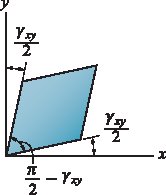
\includegraphics[height = 6cm, keepaspectratio = true]{figures/shear_block.pdf}
    \caption{Shear block diagram.}
    % \label{}
\end{figure}
We can also define shear stress as the change in angle
\begin{equation*}
    \gamma = \gamma_f - \gamma_o
\end{equation*}
\subsection{Small Strain Analysis}
Most engineering designs involve applications for which only small deformations are allowed
(i.e., \(\epsilon \ll 1\)).
Hence we can make the following approximations for the small change in angle \(\Delta{\theta}\).
\begin{align*}
    \sin{\left( \Delta{\theta} \right)} & \approx \Delta{\theta} \\
    \cos{\left( \Delta{\theta} \right)} & \approx 1              \\
    \tan{\left( \Delta{\theta} \right)} & \approx \Delta{\theta}
\end{align*}
\section{Tension and Compression Tests}
To determine the strength of a material, we must perform a tension or compression test.
This test measures the stress and strain from a load \(P\), and the results can be used to
produce a \textbf{stress-strain diagram}.
There are two ways in which the stress-strain diagram is normally described.
\subsection{Stress-Strain Diagram}
\begin{figure}[H]
    \centering
    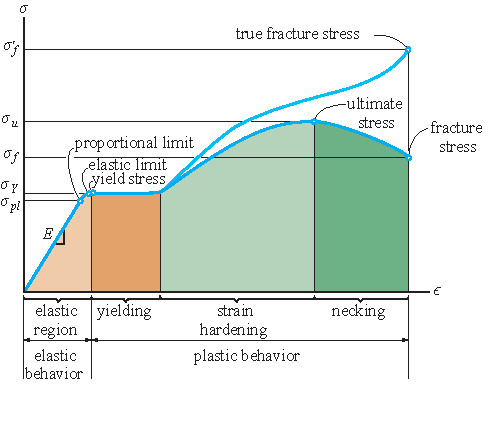
\includegraphics[height = 8cm, keepaspectratio = true]{figures/stress_strain_diagram.pdf}
    \caption{Stress-strain diagram for a typical metal.}
    % \label{}
\end{figure}
\subsubsection{Conventional Stress-Strain Diagram}
The engineering stress assumes that the area \(A\) is constant throughout
the gauge length
\begin{equation*}
    \sigma = \frac{P}{A_0}
\end{equation*}
where \(A_0\) is the \textit{original} cross-sectional area of the specimen.

Likewise, the engineering strain uses the specimen's original length \(L_0\)
\begin{equation*}
    \epsilon = \frac{\delta}{L_0}
\end{equation*}
\subsubsection{True Stress-Strain Diagram}
The true stress and true strain use the instantaneous area \(A\) and length \(L\)
at each measurement.
\subsection{Elastic Behaviour}
The initial region of the curve is referred to as the \textbf{elastic region}
where the deformation is \textit{elastic} so that unloading causes
the specimen to return to its original shape.
\subsubsection{Proportional Limit}
For the majority of the elastic deformation, the curve is \textit{linear}
up to the point where the stress reaches the \textbf{proportional limit}
at \(\left( \sigma_{pl},\, \epsilon_{pl} \right)\).
\subsubsection{Modulus of Elasticity}
The linear relationship up to this point is characterised by Hooke's law and is expressed as
\begin{equation*}
    \sigma = E \epsilon
\end{equation*}
where \(E\) is the constant of proportionality, called the \textbf{modulus of elasticity}
or \textbf{Young's modulus}.
\subsubsection{Elastic Limit}
When the stress slightly exceeds the proportionality limit,
the curve bends until the stress reaches an \textbf{elastic limit}.
\subsection{Plastic Behaviour}
An increase in stress above the elastic limit will result in a breakdown of the material
and cause it to deform plastically.
\subsubsection{Yielding}
This behaviour is called \textbf{yielding}
and the stress that causes yielding occurs at the \textbf{yield point}
\(\left( \sigma_{Y},\; \epsilon_{Y} \right)\).
Although not shown in the diagram, the yield point is distinguished as two points.

The \textbf{upper yield point} occurs first, followed by a sudden decrease in load-carrying capacity
to a \textbf{lower yield point}. Once the yield point is reached, \textit{the specimen will continue to
    elongate \textbf{without} any increase in load}. When the material behaves in this manner,
it is often referred to as being \textbf{perfectly plastic}.
\subsubsection{Yield Strength}
Commonly the proportionality limit, the elastic limit, and yield point are indistinguishable,
due to this, the \textbf{yield strength} is defined at \(\left( \sigma_{YS},\; \epsilon_{YS} \right)\).

To determine this point, a 0.2\% strain is chosen, and a line with gradient \(E\) is drawn
from the \(\epsilon\) axis.
The point where this line intersects the curve defines \(\left( \sigma_{YS},\; \epsilon_{YS} \right)\).
\subsubsection{Strain Hardening}
Yielding ends when any loading causes the stress
to increase, this rise in the curve is referred to as \textbf{strain hardening}.

When a plastically deformed ductile material is unloaded,
the elastic strain is recovered as the material returns to its equilibrium state.

However the plastic strain is maintained, resulting in a \textbf{permanent set}.
\begin{figure}[H]
    \centering
    \begin{subfigure}[H]{0.49\linewidth}
        \centering
        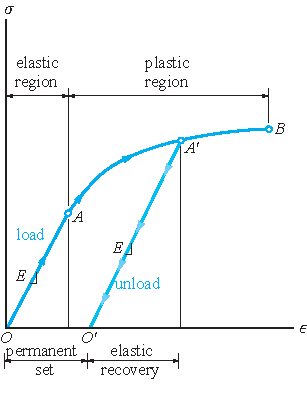
\includegraphics[height = 8cm, keepaspectratio = true]{figures/strain_hardening.pdf}
        \caption{During loading.}
    \end{subfigure}
    \begin{subfigure}[H]{0.49\linewidth}
        \centering
        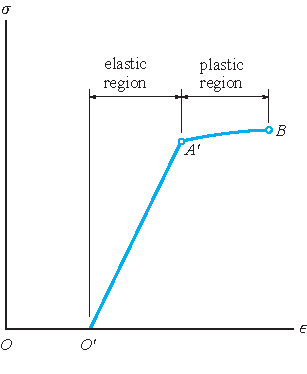
\includegraphics[height = 8cm, keepaspectratio = true]{figures/strain_hardening_recovery.pdf}
        \caption{After loading.}
    \end{subfigure}
    \caption{Elastic strain recovery under strain hardening.}
    % \label{}
\end{figure}
\subsubsection{Ultimate Tensile Stress}
The maximum stress reached on the diagram is referred to as the \textbf{ultimate tensile stress} \(\left( \sigma_{UTS},\; \epsilon_{UTS} \right)\).
\subsubsection{Necking}
While the specimen elongates up to \(\epsilon_{UTS}\), its cross-sectional area will decrease \textit{uniformally} over its gauge length.
However after reaching \(\epsilon_{UTS}\), the cross-sectional area will decrease \textit{locally}, causing an increase in stress.
As a result, a ``neck'' forms in this region, and the specimen experiences \textbf{necking}.
\subsubsection{Fracture Stress}
Finally, the specimen breaks where the curve ends at the \textbf{fracture point} at \(\left( \sigma_f,\; \epsilon_f \right)\).
\subsection{Allowable Stress Design}
To ensure the safety of a structural member, it is necessary to restrict the applied load
to one that is \textit{less than} what a member can support.

This is done by specifying a \textbf{factor of safety} \(\mathrm{F.S.}\) which
determines the allowable load \(F_{\mathrm{allow}}\) a member should be designed for.
\begin{equation*}
    \mathrm{F.S.} = \frac{F_{\mathrm{fail}}}{F_{\mathrm{allow}}}
\end{equation*}
Here \(F_{\mathrm{fail}}\) is found from experimental testing of the material. When the load is linearly
related to the stress, we can express the factor of safety using the ratio of failure stress and
allowable stress.
\begin{align*}
    \mathrm{F.S.} & = \frac{\sigma_{\mathrm{fail}}}{\sigma_{\mathrm{allow}}} \\
    \mathrm{F.S.} & = \frac{\tau{\mathrm{fail}}}{\tau_{\mathrm{allow}}}
\end{align*}
\subsection{Ductility}
\begin{definition}[Ductility]
    Ductility is a measure of the amount of plastic deformation a material can sustain under tensile stress before failure.

    Ductility can be measured using the \textbf{percent elongation} (in length) or \textbf{percent reduction} (in area)
    of a material.
    \begin{align*}
        \textrm{Percent Elongation} = \frac{L_f - L_0}{L_0} \qty{100}{\%} \\
        \textrm{Percent Reduction} = \frac{A_0 - A_f}{A_0} \qty{100}{\%}
    \end{align*}
    As the elastic region is very brief in most materials, ductility is often measured using the
    original length and area, rather than the length and area when the material undergoes
    plastic deformation.
\end{definition}
\subsection{Brittleness}
\begin{definition}[Brittleness]
    Brittleness describes the property of a material that fractures with little to no yielding.
\end{definition}
\subsection{Poisson's Ratio}
When a deformable body is subjected to a force, it can elongate longitudinally and also contract laterally.
The strain in the longitudinal (or axial) direction is given by
\begin{equation*}
    \epsilon_{\mathrm{long}} = \frac{\delta}{L}
\end{equation*}
and the strain in the lateral (or radial) direction is given by
\begin{equation*}
    \epsilon_{\mathrm{lat}} = \frac{\delta'}{r}
\end{equation*}
where \(\delta'\) is the change in the radius \(r\).

Consider the ratio of these two quantities \(\nu\)
\begin{equation*}
    \nu = -\frac{\epsilon_{\mathrm{lat}}}{\epsilon_{\mathrm{long}}}.
\end{equation*}
Within the elastic region, \(\nu\) will be constant, and it is referred
to as \textbf{Poisson's ratio}.

Note the negative value is introduced as the longitudinal and lateral strains have opposite signs.
\subsection{Strain Energy}
As a material is deformed under external load, the load will do external work.
This work is stored in the material as internal energy or \textbf{strain energy}.
\begin{figure}[H]
    \centering
    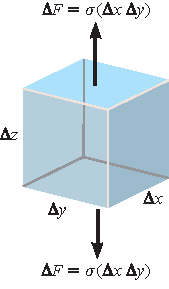
\includegraphics[height = 6cm, keepaspectratio = true]{figures/strain_energy.pdf}
    \caption{Internal energy in small element.}
    % \label{}
\end{figure}
If we consider a small volume element of the material, then the force is equal to the
average force magnitude \(\Delta F / 2\) and the displacement is given by
\(d\). Therefore the strain energy \(\Delta U\) is given by
\begin{align*}
    \Delta U & = \frac{1}{2} \Delta F d                                                               \\
             & = \frac{1}{2} \left( \sigma \Delta x \Delta y \right) \left( \epsilon \Delta z \right) \\
             & = \frac{1}{2} \sigma \epsilon \Delta V
\end{align*}
where \(\Delta V\) is the volume of the element. If we consider the strain energy
\textit{per unit volume}, then
\begin{equation*}
    u = \frac{\Delta U}{\Delta V} = \frac{1}{2} \sigma \epsilon
\end{equation*}
where \(u\) is the \textbf{strain energy density}. \(u\) can also be determined
by finding the area under the stress-strain diagram, and hence has the units \unit{J.m^{-3}}.
\subsubsection{Modulus of Resilience}
When the stress in a material reaches the
proportional limit, the strain energy density
is referred to as the modulus of resilience.
\begin{equation*}
    u_r = \frac{1}{2} \sigma_{pl} \epsilon_{pl} = \frac{1}{2} \frac{\sigma_{pl}^2}{E}
\end{equation*}
The modulus of resilience is also the area under the proportional region of the stress-strain
diagram.
\begin{figure}[H]
    \centering
    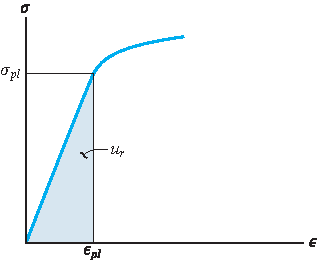
\includegraphics[height = 6cm, keepaspectratio = true]{figures/modulus_of_resilience.pdf}
    \caption{Modulus of resilience \(u_r\).}
    % \label{}
\end{figure}
\subsubsection{Modulus of Toughness}
Another important property of a material is its modulus of toughness, \(u_t\). This
quantity represents the entire area under the stress-strain diagram.
\begin{figure}[H]
    \centering
    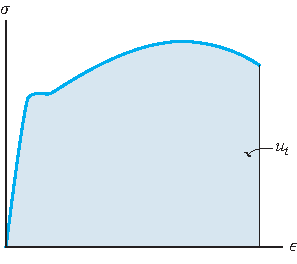
\includegraphics[height = 6cm, keepaspectratio = true]{figures/modulus_of_toughness.pdf}
    \caption{Modulus of toughness \(u_t\).}
    % \label{}
\end{figure}
\section{Shear Stress-Strain Diagram}
Similar to a tensile test, we can use a thin tube and subject
it to torsional loading. Using the data for the applied torque and resulting
angle of twist, we can form a shear stress-strain diagram.
\begin{figure}[H]
    \centering
    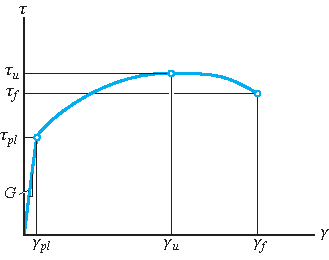
\includegraphics[height = 8cm, keepaspectratio = true]{figures/shear_stress_strain_diagram.pdf}
    \caption{Shear stress-strain diagram.}
    % \label{}
\end{figure}
\subsection{Elastic and Plastic Regions}
The curve will have similar properties to the stress-strain curve,
including the elastic and plastic deformation regions.
\subsection{Shear Modulus}
Within the proportional region of the curve, the elastic behaviour
is linear, so we can apply Hooke's law for shear to obtain
\begin{equation*}
    \tau = G \gamma
\end{equation*}
where \(G\) is called the \textbf{shear modulus of elasticity} or the \textbf{modulus of rigidity}.
\subsection{Relationship between \texorpdfstring{\(E\)}{E}, \texorpdfstring{\(G\)}{G}, and \texorpdfstring{\(\nu\)}{v}}
The three material constants, \(E\), \(G\), and \(nu\) can be related by the equation:
\begin{equation*}
    G = \frac{E}{2\left( 1 + \nu \right)}
\end{equation*}
\section{Forces}
\subsection{Rigid Body Forces and Moments}
\begin{definition}[Resultant force]
    In a system of \(n\) concurrent forces, the resultant force vector \(\symbf{F}_R\) is given by
    \begin{equation*}
        \symbf{F}_R = \sum_{i = 1}^n \symbf{F}_i
    \end{equation*}
\end{definition}
\begin{definition}[Moment]
    When a force is applied to a body it will cause the body
    to rotate about a point that is not on the line of action of the force.
    This tendency is called the moment of a force.

    The direction of the rotation is also known as the sense of direction of \(\symbf{M}_O\).

    A moment is a vector quantity measured in Newton metres (\unit{N.m}).
\end{definition}
\begin{definition}[Resultant moment]
    In a system of \(n\) concurrent forces, the resultant moment vector \(\symbf{M}_R\) about a point \(O\) is given by
    \begin{equation*}
        \left( \symbf{M}_R \right)_{O} = \sum_{i = 1}^n \left( \symbf{M}_O \right)_i
    \end{equation*}
\end{definition}
\subsubsection{Moments --- Scalar Formulation}
The magnitude of a moment about the point \(O\) can be determined using the formula
\begin{equation*}
    \norm{\symbf{M}_O} = \norm{\symbf{F}} d
\end{equation*}
where \(\symbf{F}\) acts perpendicular to a line with distance \(d\).
\begin{figure}[H]
    \centering
    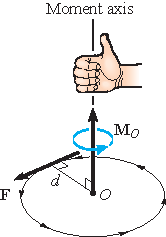
\includegraphics[height = 5cm, keepaspectratio = true]{figures/moment_scalar_perpendicular.pdf}
    \caption{Moment scalar formulation when \(\symbf{F}\) is perpendicular.} % \label{}
\end{figure}
When the force is not perpendicular to the distance,
we can use the \textbf{sliding vector} \(\symbf{r}\) along with the angle between the two vectors to determine
the magnitude of the moment.
\begin{equation*}
    \norm{\symbf{M}_O} = \norm{\symbf{F}} \norm{\symbf{r}} \sin{\left( \theta \right)}
\end{equation*}
\begin{figure}[H]
    \centering
    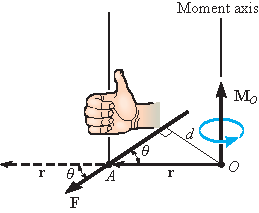
\includegraphics[height = 5cm, keepaspectratio = true]{figures/moment_scalar.pdf}
    \caption{Moment scalar resolution when \(\symbf{F}\) is not perpendicular.} % \label{}
\end{figure}
This results in the relationship
\begin{equation*}
    d = \norm{\symbf{r}} \sin{\left( \theta \right)}
\end{equation*}
\subsubsection{Moments --- Vector Formulation}
Using the vector \(\symbf{r}\) with the force \(\symbf{F}\) we can define a relationship for the moment \(\symbf{M}_O\)
\begin{equation*}
    \symbf{M}_O = \symbf{r} \times \symbf{F}
\end{equation*}
where the sense of direction is determined through the right-hand rule.
\begin{theorem}[Principle of transmissibility]
    Any position vector \(\symbf{r}\) from the point \(O\) to any point on the line of action of the force \(\symbf{F}\)
    will yield the same moment vector \(\symbf{M}_O\).
    \begin{equation*}
        \symbf{M}_O = \symbf{r}_1 \times \symbf{F} = \symbf{r}_2 \times \symbf{F} = \symbf{r}_3 \times \symbf{F}
    \end{equation*}
    \begin{figure}[H]
        \centering
        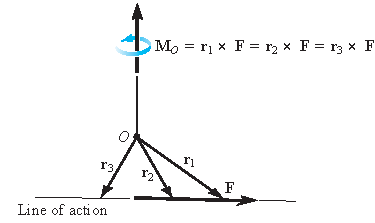
\includegraphics[height = 5cm, keepaspectratio = true]{figures/principle_of_transmissibility.pdf}
        \caption{Principle of transmissibility.} % \label{}
    \end{figure}
\end{theorem}
\begin{theorem}[Principle of moments]
    The moment of a force \(\symbf{F}\) about a point \(O\) is equal to the sum of the
    moments of the components of the force about the same point.
    \begin{equation*}
        \symbf{M}_O = \symbf{r} \times \symbf{F} = \symbf{r} \times \left( \symbf{F}_1 + \symbf{F}_2 \right) = \symbf{r} \times \symbf{F}_1 + \symbf{r} \times \symbf{F}_2
    \end{equation*}
    \begin{figure}[H]
        \centering
        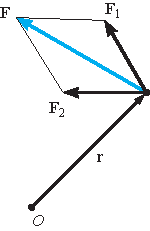
\includegraphics[height = 5cm, keepaspectratio = true]{figures/principle_of_moments.pdf}
        \caption{Principle of moments.} % \label{}
    \end{figure}
\end{theorem}
\subsection{Couples}
\begin{definition}[Couple]
    A couple is defined as two parallel forces that have the same magnitude,
    but opposite directions, that are separated by a perpendicular distance \(d\).

    Since the resultant force is zero, the only effect of a couple is to
    produce a rotation.
\end{definition}
The moment produced by a couple is called a \textit{couple moment}. We can
determine its value by finding the sum of the moments of both couple forces
about any arbitrary point.
\begin{figure}[H]
    \centering
    \begin{subfigure}[H]{0.49\linewidth}
        \centering
        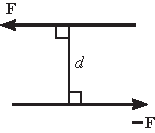
\includegraphics[height = 5cm, keepaspectratio = true]{figures/couple_2d.pdf}
        \caption{In 2d.}
    \end{subfigure}
    \begin{subfigure}[H]{0.49\linewidth}
        \centering
        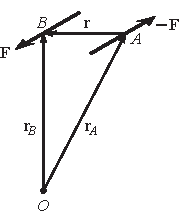
\includegraphics[height = 5cm, keepaspectratio = true]{figures/couple.pdf}
        \caption{In 3d.}
    \end{subfigure}
    \caption{Moment of a couple.} % \label{}
\end{figure}
The figures above illustrate how this moment can act at \textit{any point}
since \(\symbf{M}\) depends \textit{only} on the position vector \(\symbf{r}\).

The couple moment is determined using
\begin{equation*}
    \symbf{M} = \symbf{r}_B \times \symbf{F} + \symbf{r}_A \times \left( -\symbf{F} \right) = \left( \symbf{r}_B - \symbf{r}_A \right) \times \symbf{F}
\end{equation*}
However, \(\symbf{r} = \symbf{r}_B - \symbf{r}_A\), so that
\begin{equation*}
    \symbf{M} = \symbf{r} \times \symbf{F}
\end{equation*}
where \(\symbf{M}\) does not require a subscript.
\begin{definition}[Resultant couple moment]
    In a system of \(n\) concurrent forces, the resultant couple moment vector \(\symbf{M}_R\) is given by
    \begin{equation*}
        \symbf{M}_R = \sum_{i = 1}^n \symbf{M}_i
    \end{equation*}
\end{definition}
In summary, we can reduce a force and couple system to a resultant force \(\symbf{F}_R\), and resultant moment \(\left( \symbf{M}_R \right)_O\)
about a point \(O\), so that
\begin{align*}
    \symbf{F}_R                  & = \sum \symbf{F}                    \\
    \left( \symbf{M}_R \right)_O & = \sum \symbf{M}_O + \sum \symbf{M}
\end{align*}
\subsection{Rigid-Body Equilibrium}
When applying the equations of equilibrium we assume that the body remains rigid and does
not deform under the applied load.
\subsection{Weight}
In a gravitational field, the gravitational force acting on an object is called its weight.
Using Newton's Law of Gravitational Attraction, with \(g = G \frac{M}{r^2}\) where \(M\) and \(r\)
are the mass and radius of the earth, we can calculate the force of gravity on an object of mass \(m\)
with
\begin{equation*}
    W = m g.
\end{equation*}
\subsection{Centre of Gravity}
In a gravitational field, each particle in a body will have a weight \(\odif{W}\).
These weights form a parallel force system, so that the resultant of the system is the total
weight of the body, which passes through a single point called the center of gravity \(G\).
\subsection{Friction}
Friction is a force \(F\) that resists the movement \(P\) between two contacting surfaces that slide relative to
one another. This force always acts tangent to the surface at the points of contact, and is directed
so that it opposes the possible or existing motion between the surfaces.
\subsubsection{Static Friction}
When the frictional force \(F\) is not great enough to balance the force \(P\),
\(F\) is called the limiting static frictional force \(F_s\) as any increase in \(P\)
will cause the object to move. This force is directly proportional to the resultant
normal force \(N\):
\begin{equation*}
    F_s = \mu_s N
\end{equation*}
where the constant of proportionality \(\mu_s\) is called the coefficient of static friction.
\subsubsection{Kinetic Friction}
If the magnitude of \(P\) is increased so that it is greater than \(F_s\), the frictional force
at the contacting surface drops to a smaller value \(F_k\), called the kinetic frictional force.
The object will then begin to slide with increasing speed. The kinetic friction force is calculated
similar to the static friction force,
\begin{equation*}
    F_k = \mu_k N
\end{equation*}
where the constant of proportionality \(\mu_k\) is called the coefficient of kinetic friction.
\section{Structural Analysis}
\subsection{Supports}
A support prevents the translation or rotation of a body by exerting a force or couple moment on the body.

The following table summarises basic supports in 2d, along with their symbols and reactions.
\begin{table}[H]
    \centering
    \begin{tabular}{c c c}
        \toprule
        \textbf{Name} & \textbf{Symbol}                                             & \textbf{Reaction} \\
        \midrule
        Cable         & \begin{tikzpicture}[baseline=(current bounding box.center)]
                            \point{a}{0}{0};
                            \support{1}{a};
                            \draw[thick, ->] (0, 0) -- (0.8, 0.4);
                            \draw[dashed] (0,0) -- ++ (0.8, 0);
                            \draw[->] (0.4, 0) arc (0:26.56505117707799:0.4);
                            \node at (0.8, 0.2) {\(\theta\)};
                        \end{tikzpicture}
                      & \(\symbf{F}\) at fixed angle \(\theta\)                                         \\[0.8cm]
        Roller        & \begin{tikzpicture}[baseline=(current bounding box.center)]
                            \point{a}{0}{0};
                            \support{2oo}{a};
                        \end{tikzpicture}
                      & \(\symbf{F}_y\)                                                                 \\[0.8cm]
        Pin           & \begin{tikzpicture}[baseline=(current bounding box.center)]
                            \point{a}{0}{0};
                            \support{1}{a};
                        \end{tikzpicture}
                      & \(\symbf{F}\)                                                                   \\[0.8cm]
        Fixed         & \begin{tikzpicture}[baseline=(current bounding box.center)]
                            \point{a}{0}{0};
                            \point{b}{1.1}{0};
                            \support{3}{a}[-90];
                            \beam{2}{a}{b}[0][0];
                        \end{tikzpicture}
                      & \(\symbf{F}\) and \(\symbf{M}\)                                                 \\
        \bottomrule
    \end{tabular}
    % \caption{} % \label{}
\end{table}
\subsection{Free Body Diagrams}
To construct a free body diagram, we can use the following steps:
\begin{enumerate}
    \item Draw outlined shape
          \begin{enumerate}
              \item Isolate body
              \item Define a coordinate system
          \end{enumerate}
    \item Show all external forces and couple moments
          \begin{enumerate}
              \item Label all known forces and moments with magnitudes and directions
              \item Label all unknown forces and moments with appropriate letters
              \item Indicate any required dimensions on body
          \end{enumerate}
\end{enumerate}
\subsection{Trusses}
A truss is a structure composed of members joined at their end points.
Using the dimensions and loads on a truss, we can apply analysis techniques
to determine the forces developed in the truss members.
\subsection{Method of Joints}
By drawing a free body diagram at each joint,
we can use the force equilibrium equations to obtain the forces acting on each joint.

Generally, this requires starting at the external force and traversing each joint
individually.

When applying the equilibrium equations assume that unknown forces
are in tension so that positive magnitudes correspond to members in tension,
and negative magnitudes correspond to members in compression.
\begin{theorem}[Determinate trusses]
    Given the number of members \(m\), joints \(j\) and reactions \(r\), the following
    relationship must hold for a statically determinate system.
    \begin{equation*}
        m = 2j - r
    \end{equation*}
\end{theorem}
\begin{figure}[H]
    \centering
    \begin{subfigure}{0.4\linewidth}
        \centering
        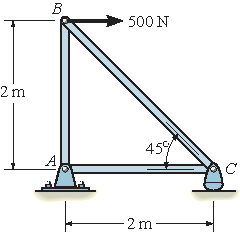
\includegraphics[width = 0.8\linewidth, keepaspectratio = true]{figures/method_of_joints_full.pdf}
        \caption{Example truss.}
    \end{subfigure}
    \begin{subfigure}{0.4\linewidth}
        \centering
        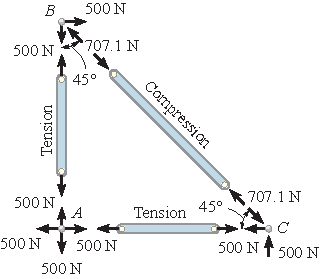
\includegraphics[width = 0.8\linewidth, keepaspectratio = true]{figures/method_of_joints_all.pdf}
        \caption{Internal forces with FBDs.}
    \end{subfigure}

    \vspace*{1.5em}
    \begin{subfigure}{0.3\linewidth}
        \centering
        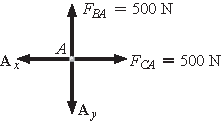
\includegraphics[height = 0.5\linewidth, keepaspectratio = true]{figures/method_of_joints_a.pdf}
        \caption{Joint \(A\) FBD.}
    \end{subfigure}
    \begin{subfigure}{0.3\linewidth}
        \centering
        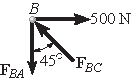
\includegraphics[height = 0.5\linewidth, keepaspectratio = true]{figures/method_of_joints_b.pdf}
        \caption{Joint \(B\) FBD.}
    \end{subfigure}
    \begin{subfigure}{0.3\linewidth}
        \centering
        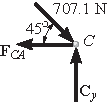
\includegraphics[height = 0.5\linewidth, keepaspectratio = true]{figures/method_of_joints_c.pdf}
        \caption{Joint \(C\) FBD.}
    \end{subfigure}
    \caption{Method of joints example.} % \label{}
\end{figure}
\subsection{Method of Sections}
To calculate the force of an arbitrary member in a truss we can utilise the method of sections.
In this method, we can create a section that cuts through a maximum of 3 members, corresponding to
the three equilibrium equations. Then the sectioned members can be treated as tension forces and
their internal forces can be determined using the equilibrium equations.
\begin{figure}[H]
    \centering
    \begin{subfigure}{\linewidth}
        \centering
        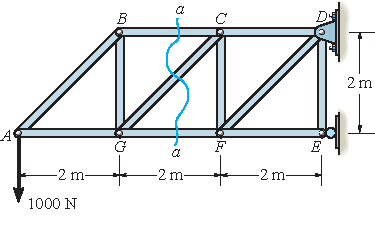
\includegraphics[height = 4cm, keepaspectratio = true]{figures/method_of_sections_full.pdf}
        \caption{Example truss.}
    \end{subfigure}

    \vspace*{1.5em}
    \begin{subfigure}{0.48\linewidth}
        \centering
        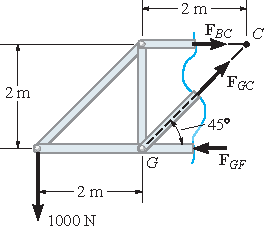
\includegraphics[height = 4cm, keepaspectratio = true]{figures/method_of_sections_left_section.pdf}
        \caption{Left section.}
    \end{subfigure}
    \begin{subfigure}{0.48\linewidth}
        \centering
        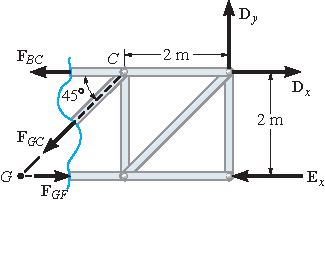
\includegraphics[height = 4cm, keepaspectratio = true]{figures/method_of_sections_right_section.pdf}
        \caption{Right section.}
    \end{subfigure}
    \caption{Method of sections example.} % \label{}
\end{figure}
\subsection{Zero Force Members}
A zero force member does not carry any load and thus has an internal force of 0.
These members are used to increase the stability of structures in the event that loading changes.

By identifying these members, we can reduce the number of members when applying the method of joints.

Zero force members can be identified by two properties:
\begin{enumerate}
    \item At a \textbf{two} member joint, if both members are \textbf{not} parallel and no external loads are
          applied at the joint, then \textbf{both} members are zero force members.
          \begin{figure}[H]
              \centering
              \begin{subfigure}{0.48\linewidth}
                  \centering
                  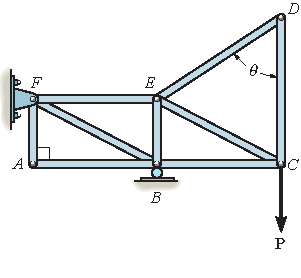
\includegraphics[height = 4cm, keepaspectratio = true]{figures/zero_force_two_member.pdf}
                  \caption{Example truss.}
              \end{subfigure}
              \begin{subfigure}{0.48\linewidth}
                  \centering
                  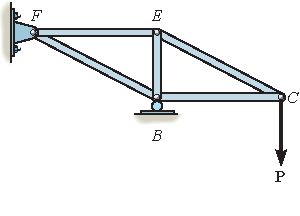
\includegraphics[height = 4cm, keepaspectratio = true]{figures/zero_force_two_member_simplified.pdf}
                  \caption{Simplified truss.}
              \end{subfigure}
              \caption{Identifying two member joint zero force members.} % \label{}
          \end{figure}
    \item At a \textbf{three} member joint, if \textbf{two} members are parallel and no external loads are
          applied at the joint, then the \textbf{third} member is a zero force member.
          \begin{figure}[H]
              \centering
              \begin{subfigure}{0.48\linewidth}
                  \centering
                  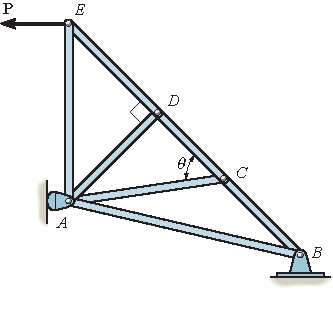
\includegraphics[height = 4cm, keepaspectratio = true]{figures/zero_force_three_member.pdf}
                  \caption{Example truss.}
              \end{subfigure}
              \begin{subfigure}{0.48\linewidth}
                  \centering
                  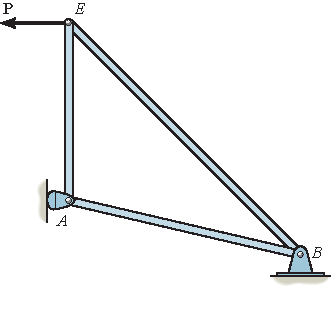
\includegraphics[height = 4cm, keepaspectratio = true]{figures/zero_force_three_member_simplified.pdf}
                  \caption{Simplified truss.}
              \end{subfigure}
              \caption{Identifying three member joint zero force members.} % \label{}
          \end{figure}
\end{enumerate}
\subsection{Frames and Machines}
Frames and machines are two types of structures which are often
composed of pin-connected multi-force members, i.e., members that are
subjected to more than two forces. Frames are used to support loads,
whereas machines contain moving parts and are designed to transmit and
alter the effect of forces.

Provided a frame or machine contains no more
supports or members than are necessary to prevent its collapse, then the
forces acting at the joints and supports can be determined by applying the
equations of equilibrium to each of its members.
\subsubsection{Free Body Diagrams}
To determine the forces acting at
the joints and supports of a frame or machine, the structure must be
disassembled and the free-body diagrams of its parts must be drawn.

The following important points must be observed:
\begin{itemize}
    \item Isolate each part by drawing its outlined shape and show all the
          forces and couple moments that act on the part.
    \item Identify all the two-force members in the structure and represent
          their free-body diagrams as having two equal but opposite collinear
          forces acting at their points of application (i.e., the pins). By doing
          this, we can avoid solving an unnecessary number of equilibrium
          equations.
    \item Forces common to any two contacting members act with equal
          magnitudes but opposite sense on the free-body diagrams of the
          respective members.
\end{itemize}
\section{Centroids}
Given the 1d region \(L:\interval{x_1}{x_2}\), 2d region \(R:\interval{x_1}{x_2}\times\interval{y_1}{y_2}\)
and 3d region \(V:\interval{x_1}{x_2}\times\interval{y_1}{y_2}\times\interval{z_1}{z_2}\),
the following definitions represent various geometric properties of a body.
\subsection{Mass}
The mass of a body with density \(\rho\) is a measure of the quantity of matter.

For a length:
\begin{equation*}
    M = \int_L \rho \odif{L}
\end{equation*}
For an area:
\begin{equation*}
    M = \iint_A \rho \odif{A}
\end{equation*}
For a volume:
\begin{equation*}
    M = \iiint_V \rho \odif{V}
\end{equation*}
\subsection{Weight}
The weight of a body is its attraction to another body (e.g., Earth),
developed by a gravitational field with acceleration \(g\).

For a length:
\begin{equation*}
    W = \int_L \rho g \odif{L}
\end{equation*}
For an area:
\begin{equation*}
    W = \iint_A \rho g \odif{A}
\end{equation*}
For a volume:
\begin{equation*}
    W = \iiint_V \rho g \odif{V}
\end{equation*}
\subsection{Centre of Mass}
The resultant mass of the particles in a body pass through a single point called the center of mass.

For a length:
\begin{equation*}
    \overline{x} = \frac{1}{M} \int_L \rho x \odif{L}
\end{equation*}
For an area:
\begin{align*}
    \overline{x} & = \frac{1}{M} \iint_A \rho x \odif{A} &  & \overline{y} = \frac{1}{M} \iint_A \rho y \odif{A}
\end{align*}
For a volume:
\begin{align*}
    \overline{x} & = \frac{1}{M} \iiint_V \rho x \odif{A} &  & \overline{y} = \frac{1}{M} \iiint_V \rho y \odif{V} &  & \overline{z} = \frac{1}{M} \iiint_V \rho z \odif{V}
\end{align*}
\subsection{Center of Gravity}
The resultant weight of the particles in a body pass through a single point called the center of gravity.

For a length:
\begin{equation*}
    \overline{x} = \frac{1}{W} \int_L \rho g x \odif{L}
\end{equation*}
For an area:
\begin{align*}
    \overline{x} & = \frac{1}{W} \iint_A \rho g x \odif{A} &  & \overline{y} = \frac{1}{W} \iint_A \rho g y \odif{A}
\end{align*}
For a volume:
\begin{align*}
    \overline{x} & = \frac{1}{W} \iiint_V \rho g x \odif{V} &  & \overline{y} = \frac{1}{W} \iiint_V \rho g y \odif{V} &  & \overline{z} = \frac{1}{W} \iiint_V \rho g z \odif{V}
\end{align*}
\subsection{Uniform Gravitational Field}
In a uniform gravitational field where \(g \in \R\) is a constant. The weight simplifies to
\begin{equation*}
    W = Mg
\end{equation*}
and the center of mass and center gravity are equal.
\subsection{Geometric Measures}
The measure of a body represents its length in 1d, area in 2d, and volume in 3d.

For a length:
\begin{equation*}
    L = \int_L \odif{L}
\end{equation*}
For an area:
\begin{equation*}
    A = \iint_A \odif{A}
\end{equation*}
For a volume:
\begin{equation*}
    V = \iiint_V \odif{V}
\end{equation*}
\subsection{Centroids}
The geometric center of a body is known as its centroid.

For a length:
\begin{equation*}
    \overline{x} = \frac{1}{L} \int_L \symbf{r} \odif{L}
\end{equation*}
For an area:
\begin{align*}
    \overline{x} & = \frac{1}{A} \iint_A x \odif{A} &  & \overline{y} = \frac{1}{A} \iint_A y \odif{A}
\end{align*}
For a volume:
\begin{align*}
    \overline{x} & = \frac{1}{V} \iiint_V x \odif{V} &  & \overline{y} = \frac{1}{V} \iiint_V y \odif{V} &  & \overline{z} = \frac{1}{V} \iiint_V z \odif{V}
\end{align*}
\subsection{Composite Bodies}
A composite body consists of \(n\) connected ``simpler'' shaped bodies.
To determine the center of gravity of such a body, we can use the sum of individual
components:
\begin{align*}
    \overline{x} & = \frac{\sum_{i = 1}^n x A_i}{\sum_{i = 1}^n A_i} &  & \overline{y} = \frac{\sum_{i = 1}^n y A_i}{\sum_{i = 1}^n A_i}
\end{align*}
where \(A_i\) is the area of each shape.
\subsection{Distributed Loads}
A distributed load on a 1d rod of length \(L\) can be represented as a point load \(\symbf{F}_R\) applied at the position \(0 \leq \overline{x} \leq L\) on the rod.
\begin{equation*}
    \symbf{F}_R = \int_0^L w\left( x \right) \odif{x}
\end{equation*}
\subsection{Moment of Inertia}
The moment of inertia describes the resistance of a moment when a force is applied perpendicular to the axis
of rotation.

The moment of inertia about the \(x\) and \(y\) axes are given by
\begin{align*}
    I_x & = \iint_A y^2 \odif{A} \\
    I_y & = \iint_A x^2 \odif{A}
\end{align*}
and the polar moment of inertia is given by
\begin{equation*}
    J_O = I_x + I_y.
\end{equation*}
\begin{theorem}[Parallel axis theorem]
    If the moment of inertia is known about an axis passing through the centroid of a region,
    then the parallel-axis theorem can be used to find the moment of inertia about any axis
    that is parallel to the centroidal axis.
    \begin{figure}[H]
        \centering
        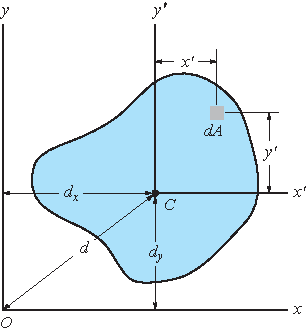
\includegraphics[height = 6cm, keepaspectratio = true]{figures/parallel_axis_theorem.pdf}
        \caption{Region with known moment of inertia about its centroidal axis.} % \label{}
    \end{figure}
    In the figure above, if \(I_{x'}\) represents the moment of inertia about the centroidal axis \(x'\),
    then the moment of inertia about the \(x\)-axis is given by
    \begin{align*}
        I_x & = \iint_R \left( y' + d_y \right)^2 \odif{A}                               \\
            & = \iint_R y'^2 \odif{A} + 2 d_y \iint y' \odif{A} + d_y^2 \iint_R \odif{A} \\
            & = \iint_R y'^2 \odif{A} + A d_y^2                                          \\
            & = I_{x'} + A d_y^2
    \end{align*}
    Similarly for \(I_{y'}\), we have
    \begin{equation*}
        I_y = I_{y'} + A d_x^2
    \end{equation*}
    so that the polar moment of inertia is given by
    \begin{equation*}
        J_O = J_C + Ad^2
    \end{equation*}
    where \(J_C = I_{x'} + I_{y'}\) and \(d^2 = d_x^2 + d_y^2\).
\end{theorem}
\section{Axial Load}
This section covers the methods used to determine the deformation of an axially loaded member.
\subsection{Saint-Venant's Principle}
The difference between the effects of two different but statically
equivalent loads becomes very small at sufficiently large distances from the load.
\subsection{Axial Deformation}
Using Hooke's Law, we can show that the axial displacement of a member is given by
\begin{equation*}
    \delta = \frac{P L}{A E}
\end{equation*}
If the member varies in cross-sectional area, elasticity, or load, then we can use the following derivation instead:
\begin{align*}
    \sigma\left( x \right)                      & = E\left( x \right) \epsilon\left( x \right) \\
    \frac{P\left( x \right)}{A\left( x \right)} & = E\left( x \right) \odv{\delta}{x}          \\
    \delta                                      & = \int_0^L \frac{P L}{A E} \odif{x}
\end{align*}
similarly for \(n\) piecewise members,
\begin{equation*}
    \delta = \sum_{i = 1}^n \frac{P_i L_i}{A_i E_i}
\end{equation*}
where we can use the method of sections and determine displacements
between changes in internal force, cross-sectional area, or elasticity.
\subsection{Principle of Superposition}
The principle of superposition is used to determine the stress or displacement
at a point in a member which is subjected to complicated loading.
By subdiving the loading into components, the resultant stress or displacement at a point
can be determined by algebraically summing the stress of displacement caused by each
load component applied separately to the member.

The following two conditions must be satisfied:
\begin{enumerate}
    \item The loading must be linearly related to the stress or displacement.
          For example, \(\sigma = P/A\) or \(\delta = PL/\left( AE \right)\),
          but not \(\sigma = P^2/A\) or \(\delta = \sin{\left( P \right)}L/\left( AE \right)\).
    \item The loading must not significantly change the original geometry or
          configuration of the member. This is because the moment
          caused by each load will not equal the resultant moment.
\end{enumerate}
\subsection{Statically Indeterminate Axially Loaded Members}
If a system is statically indeterminate, we can establish an additional \textbf{kinematic condition} that considers
the displacement of a particular point on the bar. For example, if both ends of the bar are fixed, then the following
equation may be used:
\begin{equation*}
    \delta_{AB} = 0.
\end{equation*}
\section{Shear Force \& Bending Moment Diagrams}
Members that are slender and support loadings that are applied perpendicular to their longitudinal axis are called
beams. Beams can be supported in a number of ways, the most common are:
\begin{itemize}
    \item Simply supported (pin and roller)
    \item Cantilever (fixed and hanging)
    \item Overhanging (pin and roller with roller side hanging)
\end{itemize}
The shear force and bending moment along the length of a beam can be described as functions of distance \(x\) along the beam.
We can use these functions to develop shear force and bending moment diagrams.
\subsection{Beam Positive Sign Convention}
When applying the method of sections along a beam, we start from the left side and move toward the right side of the beam.
The following sign conventions apply:
\begin{itemize}
    \item Positive loads point upwards
    \item Positive shear forces point downwards (reverse if starting from the right)
    \item Positive moments rotate anticlockwise (reverse if starting from the right)
\end{itemize}
This is illustrated on the following diagram.
\begin{figure}[H]
    \centering
    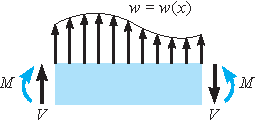
\includegraphics[height = 4cm, keepaspectratio = true]{figures/sfd_bmd.pdf}
    \caption{Positive sign convention on a section of a beam.} % \label{}
\end{figure}
\subsection{Determining the Shear Force and Bending Moment}
In each section, the length of the beam is treated as a variable \(x\),
allowing us to determine \(V\) and \(M\) for the \(i\)th section
on the interval \(s_i < x \leq s_{i + 1}\).
By constructing the piecewise function comprising of the entire length of the beam, we can
determine the shear force and bending moment diagrams.
\subsection{Determining the Shear Force and Bending Moment Analytically}
If we consider the following segment \(\Delta{x}\) on a beam of length \(L\):
\begin{figure}[H]
    \centering
    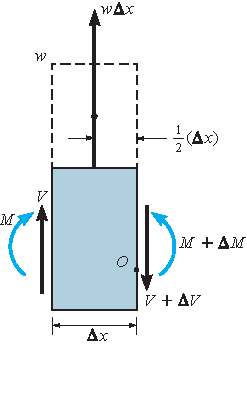
\includegraphics[height = 8cm, keepaspectratio = true]{figures/sfd_bmd_analytic.pdf}
    \caption{Small section of a beam.} % \label{}
\end{figure}
then by the equilibrium of forces in the vertical direction:
\begin{equation*}
    V\left( x \right) = \int w\left( x \right) \odif{x}
\end{equation*}
similarly the equilibrium of moments about \(O\) give:
\begin{equation*}
    M\left( x \right) = \int V\left( x \right) \odif{x}
\end{equation*}
\subsection{Point Loads}
The result of a point load \(\symbf{F}\) on a beam is a step on the shear force diagram in the direction of \(\symbf{F}\),
\subsection{Point Moments}
The result of a clockwise moment \(\symbf{M}_O\) applied at a point O on a beam is a step on the bending
moment diagram, where clockwise moments are positive.
\subsection{Bending Deformation}
Consider the following beam under bending
\begin{figure}[H]
    \centering
    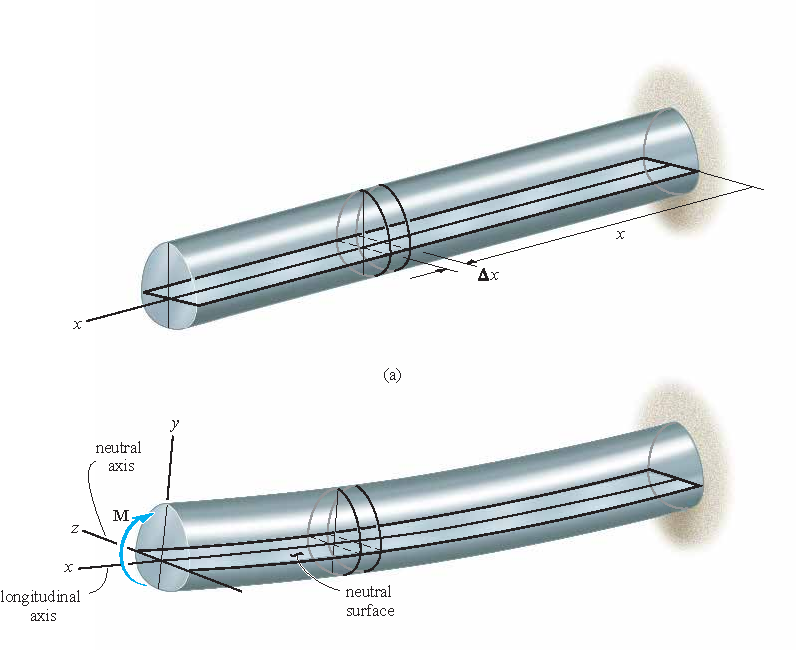
\includegraphics[height = 7cm, keepaspectratio = true]{figures/bending_deformation_diagram.pdf}
    \caption{Beam under bending deformation.} % \label{}
\end{figure}
with the following section
\begin{figure}[H]
    \centering
    \begin{subfigure}[c]{0.47\linewidth}
        \centering
        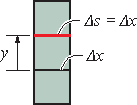
\includegraphics[height = 3cm, keepaspectratio = true]{figures/beam_section_before_bending.pdf}
        \caption{Before deformation.}
    \end{subfigure}
    \begin{subfigure}[c]{0.47\linewidth}
        \centering
        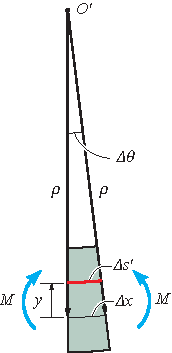
\includegraphics[height = 6cm, keepaspectratio = true]{figures/beam_section_after_bending.pdf}
        \caption{After deformation.}
    \end{subfigure}
    \caption{Beam section.} % \label{}
\end{figure}
where \(\rho\) is the radius of curvature of the beam and \(\Delta{x}\), located on the neutral surface, does not change in length
whereas \(\Delta{s}\) located at an arbitrary distance \(y\) above the neutral axis, contracts to \(\Delta{s}'\) through deformation.

By definition, the normal strain along \(\Delta{s}\) is given by
\begin{equation*}
    \epsilon = \lim_{\Delta{s} \to 0} \frac{\Delta{s}' - \Delta{s}}{\Delta{s}}
\end{equation*}
Before deformation, we have
\begin{equation*}
    \Delta{x} = \Delta{s} = \rho \Delta{\theta}
\end{equation*}
through trigonometry, we can also show that for small angles
\begin{equation*}
    \Delta{s}' = \left( \rho - y \right) \sin{\left( \Delta{\theta} \right)} \approx \left( \rho - y \right) \Delta{\theta}
\end{equation*}
therefore the above equation becomes
\begin{align*}
    \epsilon & = \lim_{\Delta{\theta} \to 0} \frac{\left( \rho - y \right) \Delta{\theta} - \rho \Delta{\theta}}{\rho \Delta{\theta}} \\
             & = - \frac{y}{\rho}.
\end{align*}
As \(\frac{1}{\rho}\) is constant at \(x\), the longitudinal normal strain will vary linearly with \(y\) measured from the neutral axis.
Therefore at distance \(y = c\) from the neutral axis the strain will be maximised.
\begin{figure}[H]
    \centering
    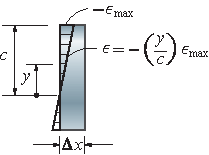
\includegraphics[height = 5cm, keepaspectratio = true]{figures/beam_strain.pdf}
    \caption{Linear strain in beam.} % \label{}
\end{figure}
Here
\begin{equation*}
    \epsilon_{\text{max}} = \frac{c}{\rho}
\end{equation*}
so that
\begin{align*}
    \frac{\epsilon}{\epsilon_{\text{max}}} & = \frac{-y/\rho}{c/\rho} \\
                                           & = -\frac{y}{c}.
\end{align*}
Given elastic deformation, we also have
\begin{equation*}
    \sigma = -\frac{y}{c}\sigma_{\text{max}}
\end{equation*}
\subsection{Flexure Formula}
\subsubsection{Location of the Neutral Axis}
To locate the neutral axis in Figure (x), we require the resultant force produced by the stress distribution
acting over the cross-sectional area to be equal to zero.
\begin{align*}
    \symbf{F}_R & = \sum F_x                                           \\
    0           & = \iint_A \odif{F}                                   \\
                & = \iint_A \sigma \odif{A}                            \\
                & = \iint_A -\frac{y}{c} \sigma_{\text{max}} \odif{A}  \\
                & = - \frac{\sigma_{\text{max}}}{c} \iint_A y \odif{A}
\end{align*}
as \(\frac{\sigma_{\text{max}}}{c} \neq 0\), \(\iint_A y \odif{A} = 0\).
\subsubsection{Bending Moment}
We can determine the stress in the beam if we
require the moment \(M\) to be equal to the moment produced by the stress
distribution about the neutral axis.
\begin{align*}
    \left( M_R \right)_z & = \sum M_z                                             \\
    M                    & = \iint_A y \odif{F}                                   \\
                         & = \iint_A y \sigma \odif{A}                            \\
                         & = \iint_A y \frac{y}{c} \sigma_{\text{max}} \odif{A}  \\
                         & = \frac{\sigma_{\text{max}}}{c} \iint_A y^2 \odif{A} \\
                         & = \frac{\sigma_{\text{max}}}{c} I_x 
\end{align*}
therefore, 
\begin{equation*}
    \sigma_{\text{max}} = -\frac{M c}{I_x}
\end{equation*}
and the normal stress at any distance \(y\) is given by
\begin{equation*}
    \sigma = \frac{M y}{I_x}
\end{equation*}
\end{document}
